\documentclass[portrait]{a0poster}

\usepackage{amsmath}
\usepackage{amssymb}
\usepackage{fontspec}
\usepackage{natbib}
\usepackage{graphicx}
\usepackage{xcolor}
\usepackage{lettrine}
\usepackage{flowfram}

% Macros
\newcommand{\EM}[1]{\ensuremath{\textsc{\textrm{em}}_#1}}
\newcommand{\GW}{\ensuremath{\textsc{\textrm{gw}}}}
\renewcommand{\familydefault}{\sfdefault}

% Adjust section style
\makeatletter
\renewcommand{\section}{\@startsection
{section}%                   % the name
{1}%                         % the level
{0mm}%                       % the indent
{-\baselineskip}%            % the before skip
{0.5\baselineskip}%          % the after skip
{\fontspec{Marvel Bold}\Huge}} % the style
\makeatother

% Expand space between lines
\linespread{1.2}

% Increase paragraph indentation
\setlength{\parindent}{4em}

% Flow frames
\newstaticframe{\textwidth}{0.3\textheight}{0\textwidth}{0.5\textheight}[title-drawing]
\newstaticframe{0.32\textwidth}{0.15\textheight}{0.34\textwidth}{0\textheight}[efficiency_distance]
\newstaticframe{0.32\textwidth}{0.15\textheight}{0.68\textwidth}{0\textheight}[efficiency_histogram]
\newstaticframe{0.32\textwidth}{0.15\textheight}{0.34\textwidth}{0.85\textheight}[convergence]
\newstaticframe{0.32\textwidth}{0.32\textwidth}{0\textwidth}{0\textheight}[healpix-dots]
\newstaticframe{0.66\textwidth}{0.025\textheight}{0.34\textwidth}{0.7\textheight}[ligosmile]
\newflowframe{0.32\textwidth}{0.025\textheight}{0.34\textwidth}{0.35\textheight}
\newflowframe{0.32\textwidth}{0.2\textheight}{0.34\textwidth}{0.15\textheight}
\newflowframe{0.32\textwidth}{0.2\textheight}{0.68\textwidth}{0.15\textheight}
\newflowframe{0.32\textwidth}{0.5\textheight}{0\textwidth}{0.5\textheight}


\begin{document}
\fontspec{Corbel}

\begin{staticcontents*}{title-drawing}

\includegraphics[width=\textwidth,clip=true,trim=0cm 5cm 0cm 0cm]{title-drawing.pdf}
\end{staticcontents*}

\begin{staticcontents*}{efficiency_distance}
\includegraphics[width=\textwidth]{../efficiency_distance}
\end{staticcontents*}

\begin{staticcontents*}{efficiency_histogram}
\includegraphics[width=\textwidth]{../efficiency_histogram}
\end{staticcontents*}

\begin{staticcontents*}{convergence}
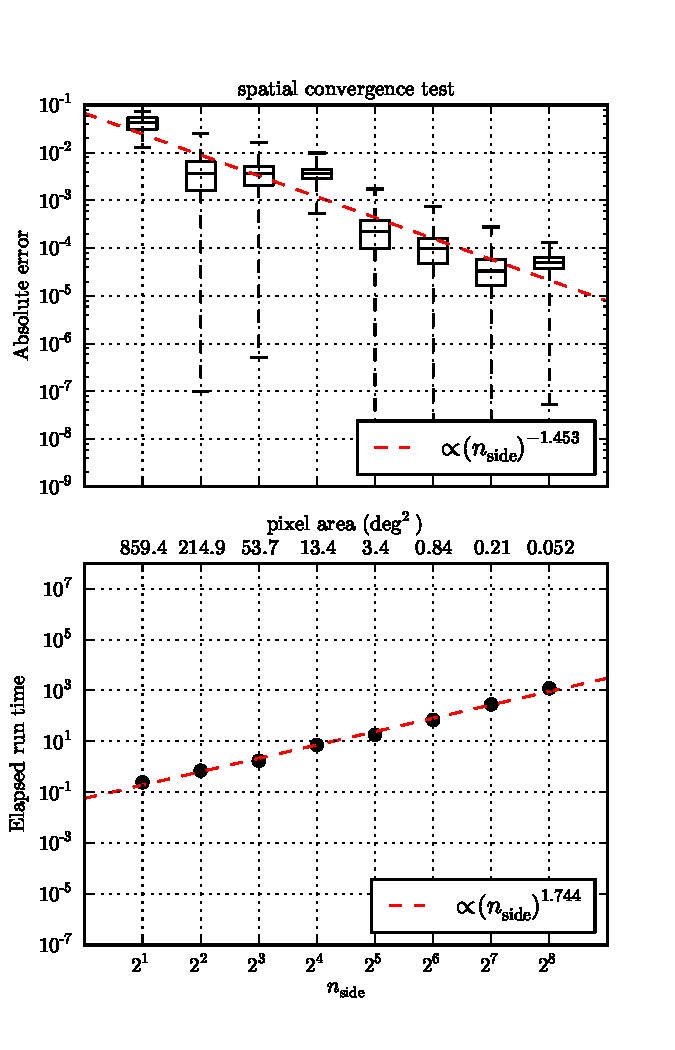
\includegraphics[width=0.5\textwidth]{spatial}
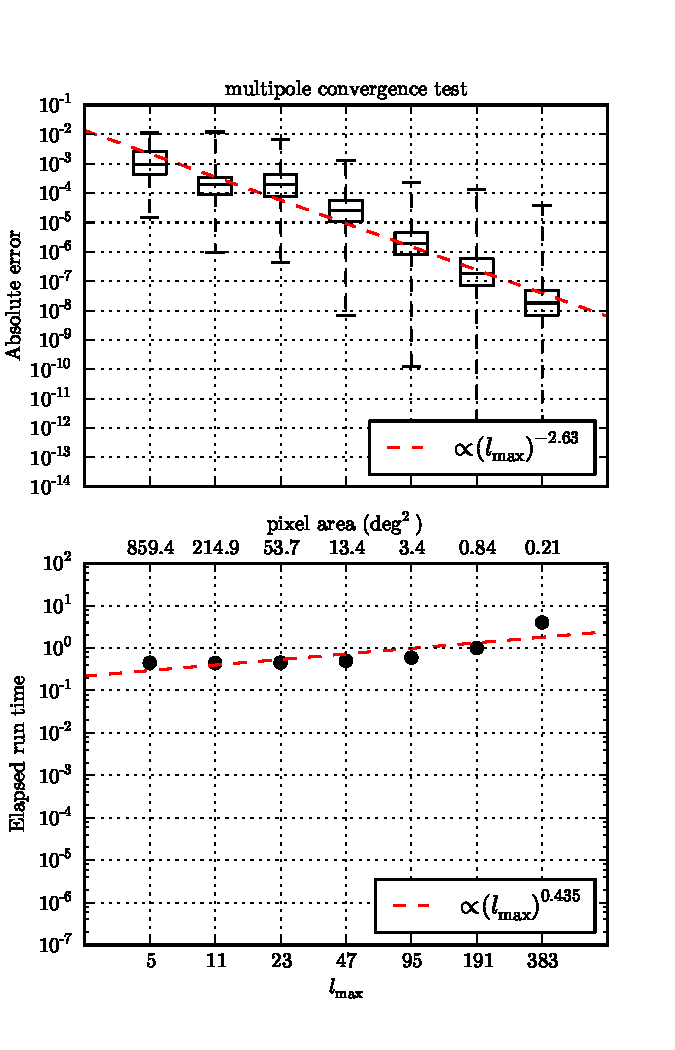
\includegraphics[width=0.5\textwidth]{multipole}
\end{staticcontents*}

\begin{staticcontents*}{healpix-dots}
\large\centering
figure 6d of~\citet{healpix}\\\vspace{5mm}
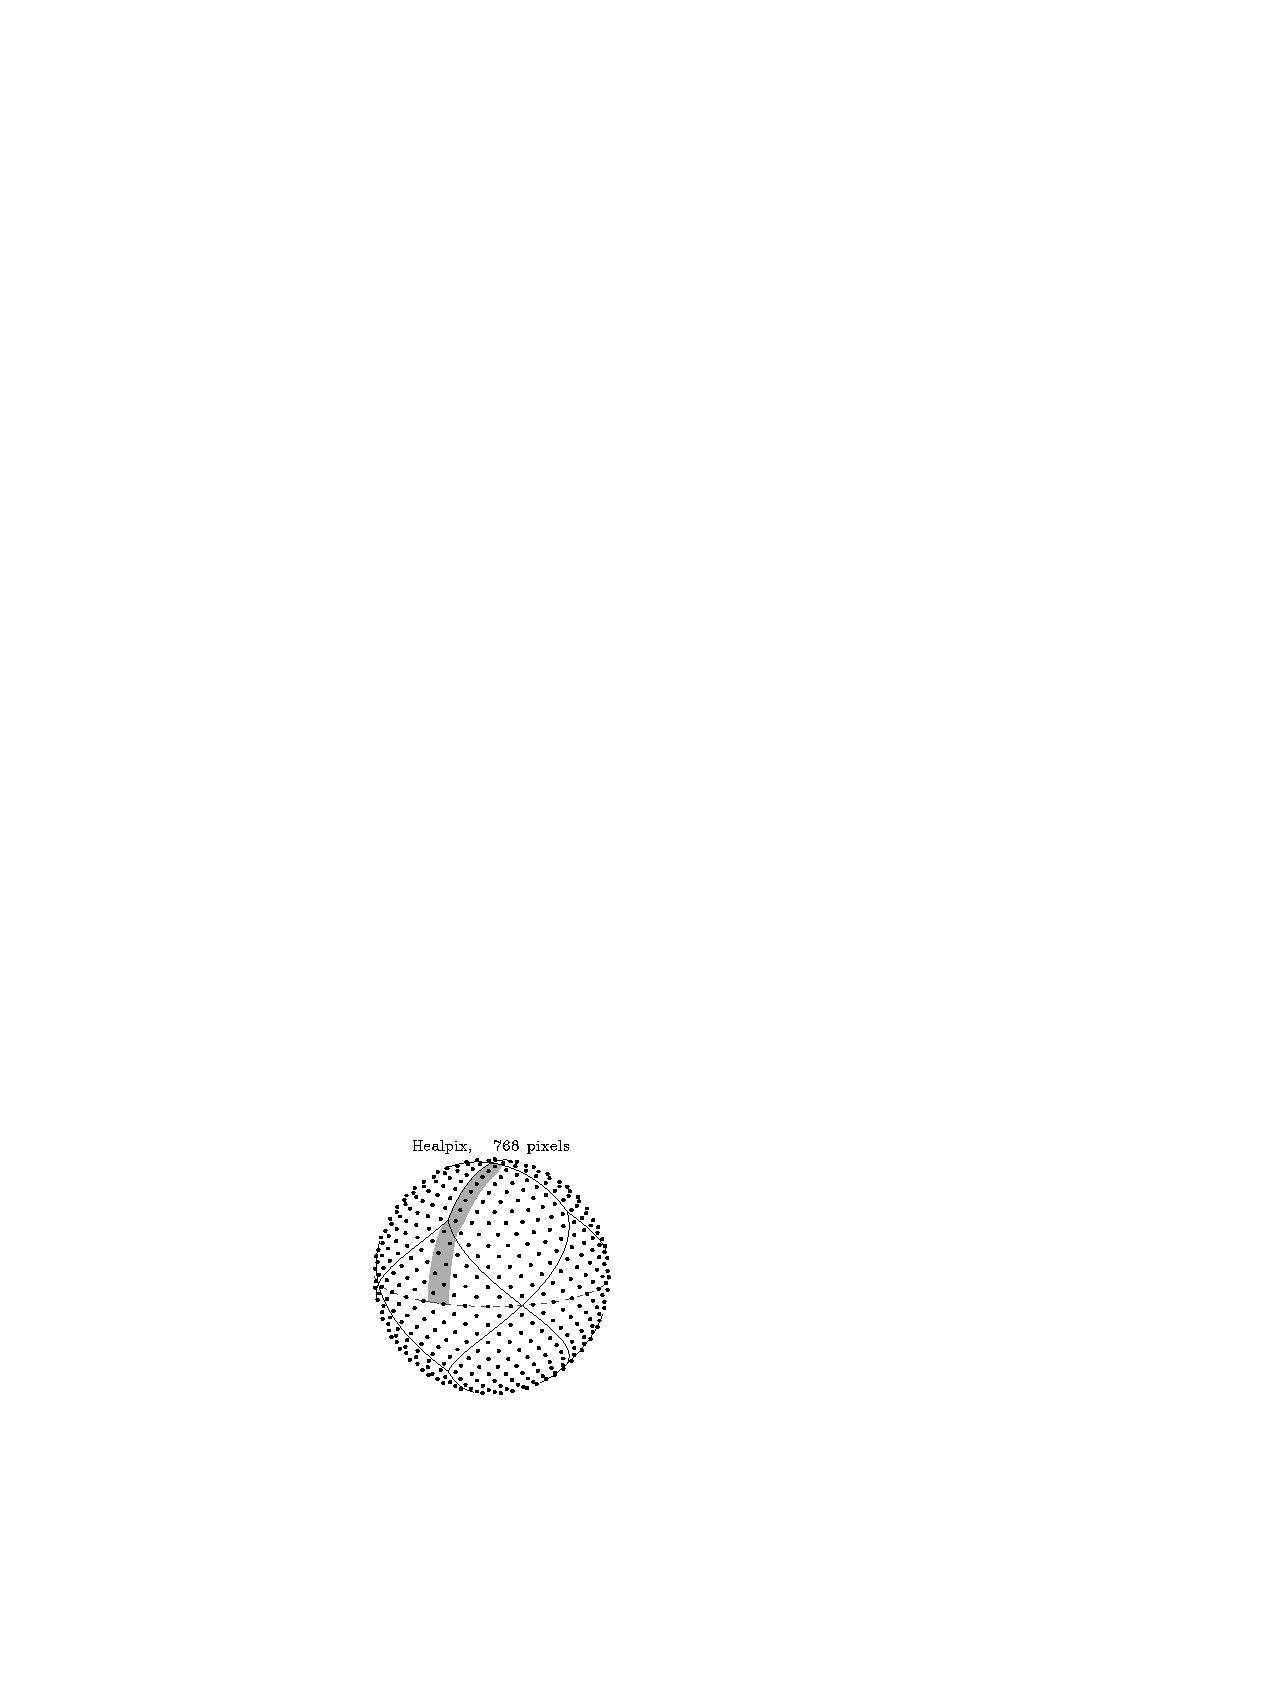
\includegraphics[width=\textwidth]{healpix-dots}
\end{staticcontents*}

\begin{staticcontents*}{ligosmile}
\begin{tabular}{ccccc}
\begin{minipage}[c]{0.3\textwidth}
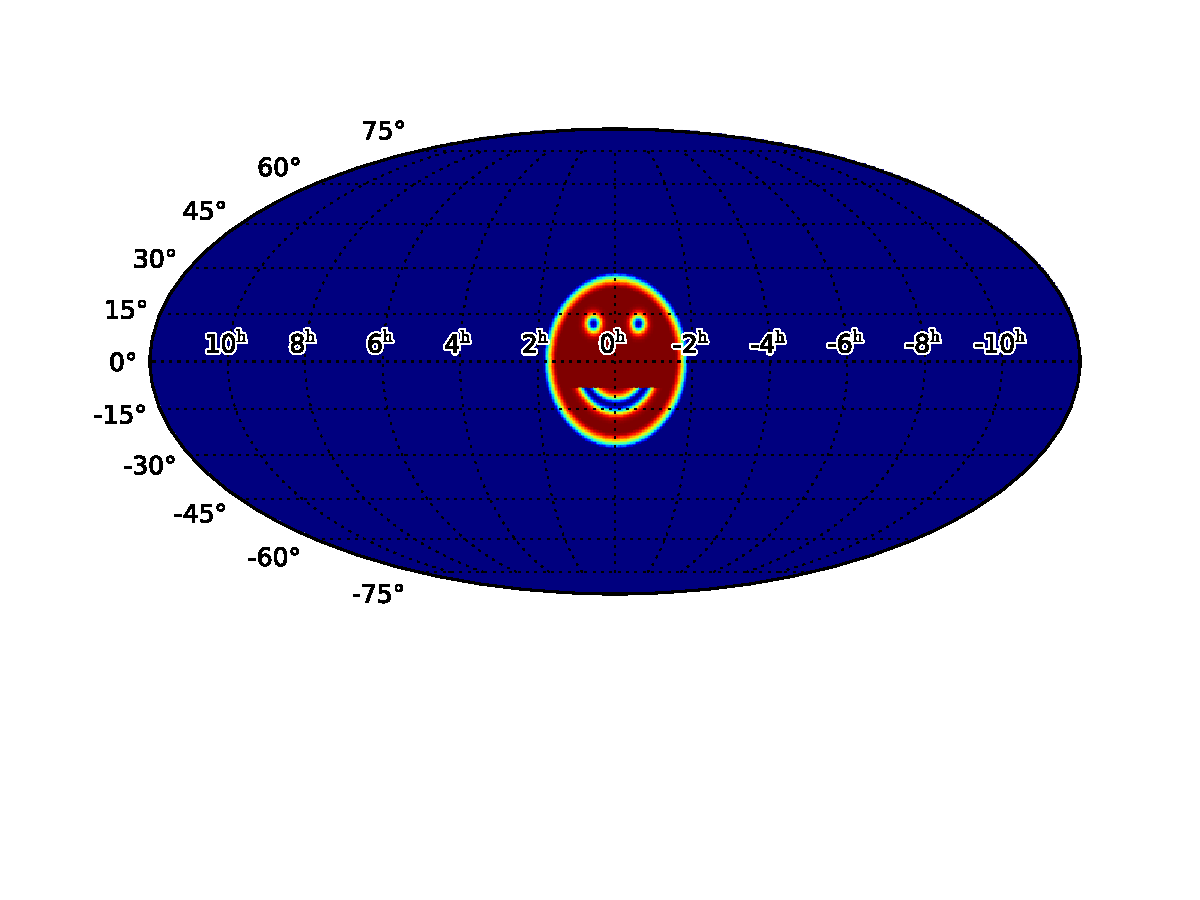
\includegraphics[width=\textwidth]{smile}
\end{minipage} &
{\Huge$\star$} &
\begin{minipage}[c]{0.3\textwidth}
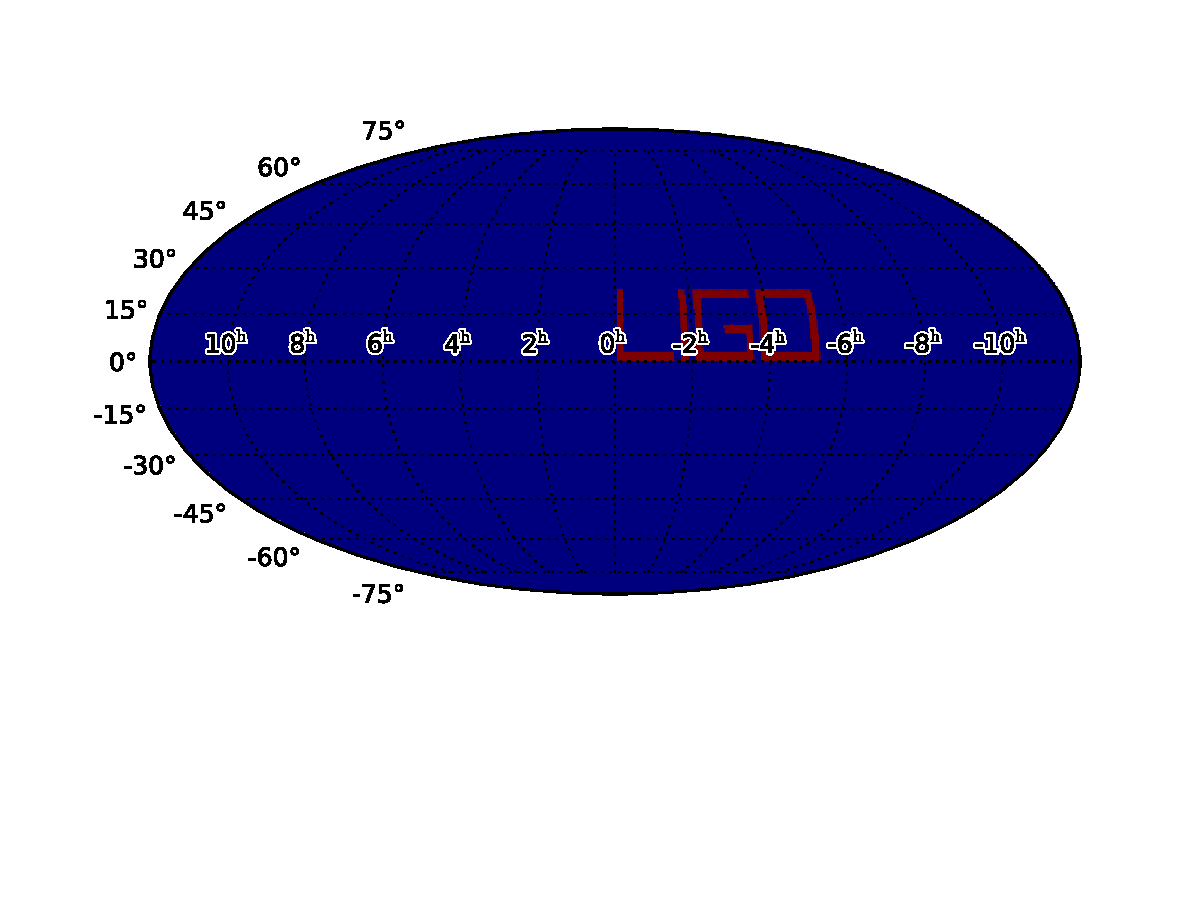
\includegraphics[width=\textwidth]{ligo}
\end{minipage} &
{\Huge$=$} &
\begin{minipage}[c]{0.3\textwidth}
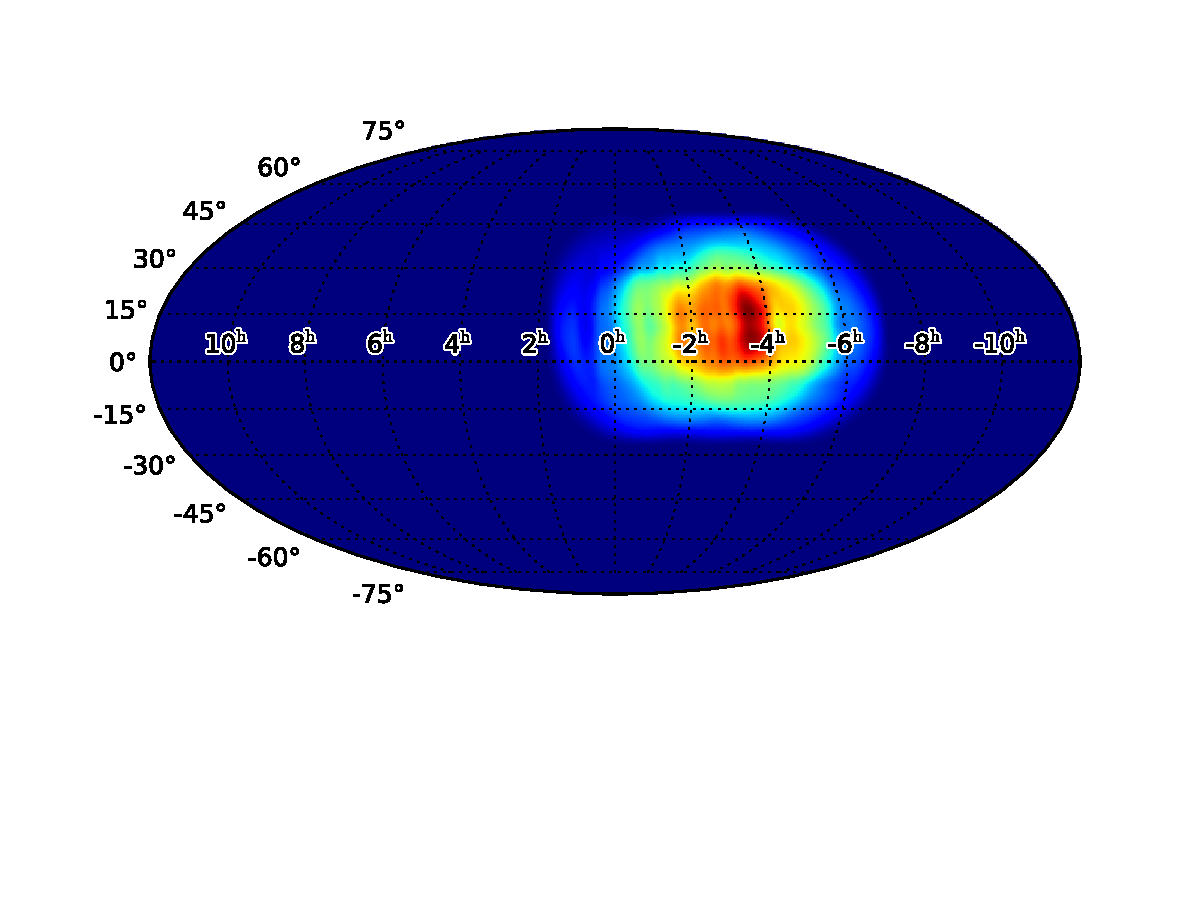
\includegraphics[width=\textwidth]{ligosmile}
\end{minipage} \\
{\fontspec{Marvel Bold}\huge Field of view} &
&
{\fontspec{Marvel Bold}\huge GW sky map} &
&
{\fontspec{Marvel Bold}\huge Cross-correlation}
\end{tabular}
\end{staticcontents*}

\section*{Background}

\framebreak

\lettrine{\fontspec{Copse}P}{\textnormal{lanning}} telescope pointings for followup of gravitational wave (GW) events is a challenging optimization problem.  Probability maps conditioned on GW observations (GW sky maps) are multimodal and dispersed over 4π.

A telescope’s field of view (FOV) may have gaps between CCDs, dead CCDs, or vignetted or clipped regions.  Any of these complications make it harder to decide on the “best” place to point a telescope.

We realized that we could phrase the single telescope problem in terms of a cross-correlation of the telescope’s FOV and the GW sky map and attack it with HEALPix, the workhorse of CMB mapping, and harmonic analysis on the sphere.

Our summer student (A. Speranza) implemented the fast convolution of~\citet{Wandelt:2001p13439} and used it to evaluate the probability of imaging an EM counterpart as a function of the source’s distance.  As we expected, the harmonic analysis algorithm was much faster than the spatial algorithm.

What surprised us was that coordinating all of the observations by maximizing the probability of imaging the source conditioned on all of the telescopes’ pointings \emph{doubled} the number of detectable sources as compared to deciding each telescope’s configuration in isolation.

\framebreak

Our key results are the two figures below.  At left is the fraction of injected signals that we would have imaged with one pointing of each telescope at the time of the trigger as a function of luminosity distance.  Solid lines represent observing plans that account for interference from the Sun and Earth.  Dashed lines represent observing plans in which these considerations are neglected.

We tested three different planning algorithms:

\paragraph{\color{red}noncooperative}
Each telescope is independently pointed where it is most likely to observe an EM counterpart.

\paragraph{\color{green!50!black}greedy sorted}
Suppose that we have chosen pointings for telescopes 1, 2, $\dots$, $i$.  The pointing of telescope $i+1$ is chosen to maximize the probability of detection, subject to telescopes 1, 2, $\dots$, $i$, remaining fixed.

\paragraph{\color{blue}anneal}
Uses simulated annealing to the probability of imaging the source by varying the configurations of all of the telescopes simultaneously.

\framebreak

\section*{Single telescope case}

\lettrine{\fontspec{Copse}F}{\textnormal{or}} GW detectors, the observables are strain time series.  The GW sky map, is the posterior distribution
$$
	p(\omega | \GW) = s(\omega)
$$
where $\omega$ is the source location and $\GW$ denotes all GW observations.  Let $\EM{i}$ denote the event of observing an optical transient with telescope $i$.  Let $C_i$ represent the configuration of telescope $i$, which consists of a pointing orientation $\gamma_i$.  The probability of observing an EM counterpart in telescope $i$ given its pointing $\gamma_i$ is
$$
	p(\EM{i} | \gamma_i, \omega) = b_i(\gamma_i^{-1} \omega).
$$
Now, marginalizing over the unknown source location, this becomes
$$
	p_i \equiv p (\EM{i} | \gamma_i, \GW) = \int s(\omega) b_i(\gamma_i^{-1} \omega) \, \mathrm{d}\Omega.
$$
The optimal pointing of a single telescope (ignoring sun and horizon interference) is
$$
	\gamma_i^* = \arg \max_{\gamma_i} p(\EM{i} | \gamma_i, \GW).
$$
The integral strongly resembles a convolution on the unit sphere.

\section*{Multiple telescope case}

For multiple telescopes, the figure of merit is the probability of imaging the source with at least one telescope:
$$
	p_{\geqslant 1} \equiv \sum_i p_i - \sum_{i \neq j} p_{ij} + \sum_{i \neq j \neq k} p_{ijk} - \cdots
$$
This is \textbf{not} the same as the probability of imaging the source with telescope 1, or telescope 2, or telescope 3 \dots :
$$
	p_{1 \textrm{ or } 2 \textrm{ or } 3 \textrm{ or } \dots} = p_1 \, p_2 \, p_3 \dots \neq p_{\geqslant 1}
$$

\bibliographystyle{apj}
\bibliography{../proposal,../telescope,../telescope_list}

\end{document}
